\documentclass[a4paper]{article}
\usepackage[T1]{fontenc}
\usepackage[utf8]{inputenc}
\usepackage{graphicx}
\usepackage[italian]{babel}
\usepackage{float}

\begin{document}

\author{Lorenzo Dentis lorenzo.dentis@edu.unito.it, Andrea nonmiricordoildnome andrea. @edu.unito.it}
\title{Idee App ProgMob}
\maketitle

\section{WalkWithMe}
(il nome è orribile) \\ \\
L’idea è quella di fornire un “social” di aggregazione per condividere una attività sportiva all’aria aperta (passeggiata, corsa, hiking).\\
Vi sono 2 grosse funzionalità: Programmata e in real time.
\begin{itemize}
	\item Programmata: prende spunto dalla funzionalità “combiniamo qualcosa” del sito www.gulliver.it 
	\begin{figure}[H]
		\centering
		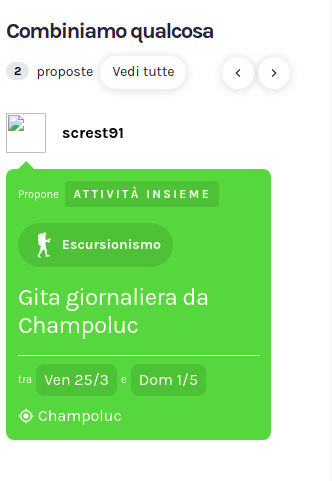
\includegraphics[scale = 0.5]{gulliver.png}
	\end{figure}
	L'idea è quella di permettere ad un utente di impostare il tipo di attività a cui è interessato a partecipare e la zone, quando un altro utente pubblica una proposta di attività del tipo correttonella zona indicata dall'utente egli riceve una notifica e l'attività viene "salvata" in una schermata apposita.\\
	C'è naturalmente la possibilità di pubblicare proposte (ed in quel caso verrano visualizzate anche le proposte "vicine") e la possibilità di "esplorare" proposte in zone geografiche diverse o attività differenti 
	\item Real time: L'utente mentre sta svolgendo una attività può effettuare broadcast della sua posizione (funzionalità ovviamente volontaria) in modo da permettere ad altri utenti di unirsi a lui qualora siano geograficamente vicini.\\
		Esempio: l'utente sta andando a funghi, inizia a fare advertising della sua posizione in combinazione con l'attività (andare a funghi). altri utenti che si trovano in prossimità, qualora fossero interessati ad andare a funghi, ricevono una notifica e sono invitati ad unirsi.

\end{itemize}
\end{document}
